% This is based on the LLNCS.DEM the demonstration file of
% the LaTeX macro package from Springer-Verlag
% for Lecture Notes in Computer Science,
% version 2.4 for LaTeX2e as of 16. April 2010https://preview.overleaf.com/public/kpngzxngmvxs/images/811041eb9a17090bad96d8e4d62cb7a6cf4adcf2.jpeg
%
% See http://www.springer.com/computer/lncs/lncs+authors?SGWID=0-40209-0-0-0
% for the full guidelines.
%

\documentclass[runningheads]{llncs}
\newcommand\tab[1][1cm]{\hspace*{#1}}
\usepackage{comment}
\usepackage{graphicx}
\usepackage{graphics}
\usepackage{subcaption}
\captionsetup{compatibility=false}
\usepackage{wrapfig}
\usepackage{algorithm,algorithmic}
\usepackage{amsmath}
\usepackage{amssymb}
\usepackage{booktabs}
\usepackage{multirow}
\usepackage[table,xcdraw]{xcolor}
\usepackage{rotating}
\usepackage[misc,geometry]{ifsym} 

% user annotations
\begin{comment}
\newcommand{\ian}[1]{\textcolor{red}{#1}}
\newcommand{\lk}[1]{\textcolor{blue}{#1}}
\newcommand{\js}[1]{\textcolor{magenta}{#1}}
\newcommand{\cc}[1]{\textcolor{teal}{#1}}
\newcommand{\rl}[1]{\textcolor{green}{#1}}
\end{comment}

%\begin{comment}
\newcommand{\ian}[1]{}   % turn off
\newcommand{\lk}[1]{}   % turn off
\newcommand{\js}[1]{}   % turn off
\newcommand{\cc}[1]{}   % turn off
\newcommand{\rl}[1]{}   % turn off
%\end{comment}


\begin{document}

\title{Vehicle Semantics Extraction and Retrieval for \\Long-term Carpark Video Surveillance}
%
%                                     also used for the TOC unless
%                                     \toctitle is used
%
\author{Clarence Weihan Cheong (\Letter) \inst{1} \and Ryan Woei-Sheng Lim\inst{1} \and
John See\inst{1} \and \\ Lai-Kuan Wong\inst{1} \and Ian K.T. Tan\inst{1} \and Azrin Aris\inst{2}}
%
\authorrunning{Cheong et al.} % abbreviated author list (for running head)
\titlerunning{Vehicle Semantics Extraction 
\& Retrieval for Long-term Surveillance}  % abbreviated title (for running head)
%
%%%% list of authors for the TOC (use if author list has to be modified)
\tocauthor{Clarence Weihan Cheong, Ryan Woei-Sheng Lim,
John See, Lai-Kuan Wong, Ian K.T. Tan, Azrin Aris}
%
\institute{Center for Visual Computing, Multimedia University,\\Persiaran Multimedia, 63100 Cyberjaya, Malaysia,\\
\email{clarence\_han@hotmail.com, ryanlim0616@gmail.com, johnsee@mmu.edu.my, lkwong@mmu.edu.my, ian@mmu.edu.my}
\and
VADS Lyfe, Telekom Malaysia Berhad, 60000 Kuala Lumpur,\\
\email{azrin.aris@tm.com.my}
}

\maketitle              % typeset the title of the contribution

\begin{abstract}
\ian{title seem to be missing the "storage" word somewhere, not sure if it is necessary} Car park video surveillance data provides plenty of semantic rich data such as vehicle color, trajectory, speed, and type which can be tapped into and extracted for video and data analytics\ian{see comment in para one of Introduction}. We present methods for extracting and retrieving color and motion semantics from long term carpark video surveillance.\ian{can remove the "However"} This is a challenging task in outdoor scenarios due to ever-changing illumination and weather conditions,\ian{this part sounds a bit odd}\js{yes, it does. modified.} while retrieval time also increases as data size grows.
%as the database size grows, longer retrieval time is required. 
To address these challenges, we subdivided\ian{"subdivided" or similar word instead of broke} the search space into smaller chunks by introducing spatio-temporal cubes or \emph{atoms}\ian{are you intending to call this ATOM or is it used somewhere else?}, which can store and retrieve these semantics at ease. The proposed method was tested on 2 days of continuous data from an outdoor carpark under various lighting and weather conditions. We report the precision, recall and $F_1$ scores to determine the overall performance of the system. %Our approach proves to be fairly accurate, and lightweight in terms of storage size.

\keywords{Vehicle Semantic Extraction, Retrieval Systems, Carpark Surveillance}
\end{abstract}
%
\section{Introduction}
%

\ian{generally clear and well presented with some parts that can be elaborated.  @John/LK, I think for MMM, maybe the area should be reduced as the work is quite comprehensive for a conference. I know, I felt the same way with Ryan's earlier paper as well.}

\ian{The "atom" stuff needs to be explained or referenced somewhere}

\ian{the overall flow is good, some sentences can be too long (I do the same thing, and usually the other Ian will point it out for me)}

\ian{try to avoid active voice, the "we", "us" etc.  This is subjective but just my personal preference}

The use of video-based \lk{video-based}traffic surveillance is becoming increasingly popular\lk{becoming increasingly popular} due to the low implementation cost. However, majority of these data are left unprocessed \lk{unprocessed}and kept in storage devices.\lk{Semantic} Rich semantic data such as vehicle color, trajectory and type \ian{what type?}can be exploited for video and data analytics \ian{keep it consistent with the first sentence in abstract - I prefer this}to provide deeper insights for surveillance and retrieval purposes.% and \lk{to ease}to ease the retrieval process. 

Traditionally,\lk{to perform} to perform retrieval on surveillance videos, users\lk{need} need to provide\lk{the} description of the vehicle such as the time, place of the incident, vehicle registration plate\ian{I think the universal term is car registration. I think "license" is colloq malaysian?}\cc{apparently license plate is an American thing },\lk{and} and color of the vehicle. \lk{Next, users need to filter through all the video retrieval results to detect the target event}Next, users would filter through all the retrieved results to manually identify 
%detect \js{changed} 
the target event. %is followed by the person-in-charge going through all the videos from the given time period trying to detect the said event.%  
This entire process is\lk{undoubtedly} undoubtedly time consuming and labor intensive.

\lk{To overcome the inefficiency of the traditional methods, we}To overcome the inefficiency of such laborious methods, %surveillance systems can extract semantics from long-spanning video footages
we propose a long-term surveillance analytics system that extracts and stores the semantics data into a database 
and allow video clips of specific events to be retrieved using user-described queries. \lk{into a database and allow video clips of specific events to be retrieved using user-described queries.} %then automates the retrieval process by taking in user described queries and returning videos clips of such events of interest. %

First, our method performs background subtraction to extract foreground blobs that represents\lk{that represents} vehicles. Next, a filtering process is applied to remove any unwanted blobs such as pedestrians\lk{as pedestrians}. They \lk{or detected vehicles}are then tracked frame by frame to generate their individual trajectories and to extract\lk{to extract} vehicle-specific semantics. Lastly, these semantics are segmented into spatio-temporal cubes (atoms) and stored in the database. We evaluated the reliability and performance of the proposed method over a span of 20 hours. \ian{this is 10 hours x 2 days right?}

%\lk{I think the following paragraph is not necessary and can be removed to save space} The remaining of this paper is organized as follow. Section 2 reviews related works on color and motion semantics extraction and retrieval from carparks. Then, Section 3 describes the framework of the proposed method.  Experimental results and conclusion are presented in Section 4 and Section 5 respectively.% 
\ian{just wondering, should the Framework section be called Framework and Implementation?}
 
 
 
\section{Related Works}
%
While Intelligent Transportation System (ITS) is a popular research topic, there has been little research done for carpark scenes. When viewed regardless of the intended scene, vehicle semantics extraction and trajectory retrieval for surveillance video is a wide research field. 

For vehicle color semantics, there are many different school of thoughts that arise from it. Authors in \cite{castanon2016retrieval} and \cite {feris2012large} approach this challenge by obtaining the histogram in HSV/HSL color space while other works \cite{dehghan2017view,hu2015vehicle,rachmadi2015vehicle} addressed it by designing deep learning methods. In an interesting work \cite{moghimi2014shadow}, color spaces were also used to detect moving shadows from urban surveillance video. 

In the area of vehicle motion extraction and trajectory grouping, the authors in \cite{zhang2013mining} and \cite{castanon2016retrieval} quantized the moving direction of the objects into 4 and 9 directional bins respectively. In \cite{d2015designing}, a novel method of indexing trajectories into spatio-temporal cubes is introduced. A recent work by Casta\~{n}\'{o}n et al. \cite{castanon2016retrieval} used other vehicle semantics such as size and persistence to query for anomalous and typical events.

\section{Framework}
\begin{figure*}[t]
  \centering
  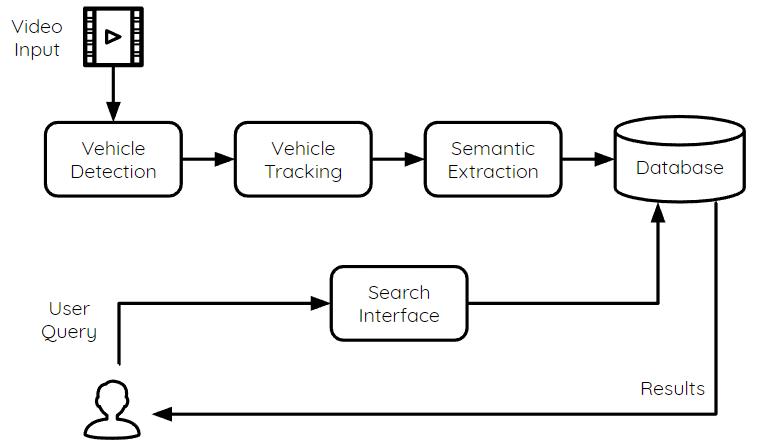
\includegraphics[width=0.7\textwidth]{Images/framework.PNG}
  \caption{Framework diagram}
  \label{fig:FDiagram}
  \vspace{-0.75em}
\end{figure*}
%\lk{Suggest to remove the first paragraph to save space} \ian{remove "Since"} The focus of this paper lies in the semantics extraction and retrieval methods, the background subtraction, object detection and tracking methods. These will be described briefly in this section.%
%\lk{Changed all "object" terms to "vehicle" to be more specific}%
The framework of our proposed method adheres to the typical top-down approach for automated video surveillance in carparks \cite{lim2017} which includes background subtraction, blob filtering, vehicle\lk{vehicle} %\lk{removed}object%
detection\lk{and vehicle} %\lk{removed}object%
vehicle tracking. The semantic information from these vehicle blobs are %\lk{removed}then %
extracted, %\lk{removed}and%
segmented into atom-based cubes and stored in the database. %\lk(removed}Finally,%
This information can then be queried through a search interface. The overview of our framework is %\lk(removed}as%
shown in Figure \ref{fig:FDiagram}. 
 
 \subsection{Background Subtraction, \lk{Vehicle}Vehicle Detection and Tracking}
We describe a number of preparatory steps that were taken prior to the extraction of semantics. Firstly, background subtraction with a combination of adaptive learning and frame differencing \cite{lim2017} is performed to extract foreground blobs from each video frame. %was chosen \ian{moved the "we chose"} 
This strategy is computationally cheaper than optical flow, %as it is computationally cheaper \ian{may help to reference this so that it is not us saying so}, 
 hence it improves on the overall efficiency of segmenting moving objects. %The foreground blobs for each frame is extracted by performing the background subtraction with a combination of adaptive background learning and frame differencing methods. 
% js: removed as not so essential to say 
%The combination of both background subtraction methods synergizes\ian{not too clear on "energizes"}\cc{typo.. synergize,updated} to balance out the shortcoming of each individual method when used alone. 

% js: verbose...
%To further improve the performance of the proposed method, 
Since the focus is on carpark surveillance where %segments \ian{"segments"?}
large portions
of the video footages may not contain any substantial movement, a frame skipping method was deployed to speed up the overall processing. The blobs then go through a series of morphological operations such as dilation and erosion\ian{removed some words} to filter out noise and to fill up gaps in the blobs to generate the final foreground blobs. 

\begin{comment}
\begin{algorithm}[!h]
  \caption{Vehicle Detection}
  \label{algo:overview}
  \begin{algorithmic}[1]
    \FOR{Each video}
    	\FOR{Each frame}
        	\STATE Extract foreground blobs 
            	\IF{No foreground blobs found}
                	\STATE Skip frame
                \ELSE
                
        			\STATE Perform morphological operations on foreground blobs
        			\STATE Model and filter foreground blobs
        			\FOR{Each previous frame's blobs}
            			\IF{Match blobs(Blob) == true}
                			\STATE Update blobs
                		\ELSE
                			\STATE Add new tracking blob
                \ENDIF
        	\ENDFOR	
            \STATE Extract Semantics
            \STATE Store data to the database
            \STATE Return final tracking blobs
            \ENDIF
    	\ENDFOR
    \ENDFOR
  \end{algorithmic}
\end{algorithm}
\end{comment}
Next, the blobs are filtered according to their sizes, positions and aspect ratios, where each of these parameters were determined empirically to suit the scene geometry. 
%It is\ian{normally, we don't shorten the words} also worth noting that these parameters are tunable %\lk{removed}accordingly%
%for other videos of different viewing perspective. 
After that, the YOLO real-time object detector \cite{redmon2016you} is applied to differentiate between %\lk{removed}identify if the final blobs belongs to%
vehicles or non-vehicle blobs.
This two-step approach is designed to filter out objects other than vehicles that are not of interest such as pedestrians and motorcycles.  Finally, each blob %\lk{removed}s are then% 
is matched back to the trajectories using a tracking state machine proposed in \cite{lim2017}. %The overview of the methods used is described in Algorithm \ref{algo:overview}.

 
\subsection{Object Specific Semantic Extraction}
%The ability to extract% 
As object specific semantics from the scene provides deeper insights for surveillance purposes%and the increases the accuracy of a search query as it is highly dependent on the information provided
, this work currently focuses on two types of object specific semantics,  
%In the following subsections, we discuss these two semantics used in the retrieval process,
namely the color and motion information. \ian{sentence kinda long}

\subsubsection{I. Color information} plays a significant role in the retrieval process as it is often one of the most common information given when a user tries to describe an object from an event in a scene. Extracting color information accurately is particularly challenging %and poses a challenge  
for outdoor scenes as the color information varies throughout the day due to ambient illumination and weather changes. Algorithm \ref{algo:colorExtract} summarizes our strategy for extracting color information.

%To address this challenge, 
When a vehicle is detected in the scene, a bounding box of the foreground blob is usually used to mark the location of the vehicle. However, due to the background subtraction method used, the final foreground blob appears slightly larger than the actual footprint of the vehicle. In order to obtain a closer estimation of the vehicle's dominant color, the bounding box is cropped by 30\% to reduce some background information such as the road or vehicles around it. %We chose not to shrink the bounding box further as it may focus on the windscreen and windows regions hence losing information and altering the overall dominant color.%

Subsequently, our strategy determines the dominant color of each vehicle blob by first undertaking a task to determine if the vehicle's dominant color belongs to the achromatic scale (black, gray and white color) or chromatic scale (other hues). 
%By comparing the cropped\ian{probably a better phrase than "shrunk down", can't think now} image against the grayscale image, 
We determine the absolute difference between the cropped image and its grayscale version, and then %Next, this value is then 
threshold each channel in RGB at an empirically-found intensity value of 35. %(approximately 14\%)\ian{is this standard or around standard?  how was this derived? or empirically tested?} 
%instead of grayscale domain as to prevent loss of information. 
The hint of significant values from this step indicates a substantial presence of chromatic hue. Then, we convert the thresholded image to a grayscale image, and determine the ratio of non-zero pixel values over total pixels. 
\begin{figure*}[t!]
\centering
\begin{subfigure}{\textwidth}
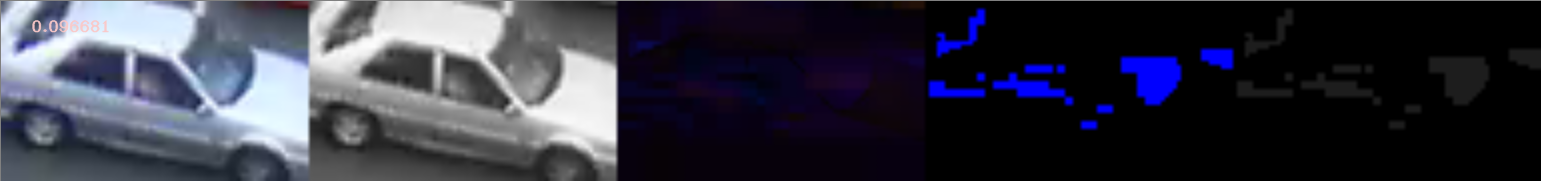
\includegraphics[width=\textwidth]{Images/achromatic_threshold5.PNG}
\caption{Achromatic vehicle (Gray/White)} \label{fig:achro_black}
\end{subfigure}
%\hspace*{\fill} 
\begin{subfigure}{\textwidth}
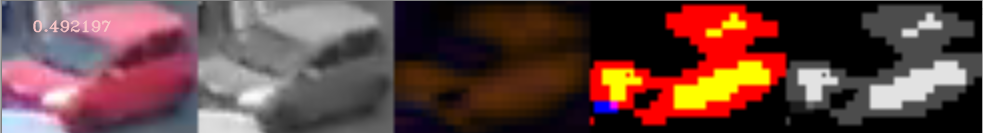
\includegraphics[width=\textwidth]{Images/achromatic_threshold_color2.PNG}
\caption{Chromatic vehicle (Red)} \label{fig:achro_red}
\end{subfigure}
%\hspace*{\fill} 
%\vspace{-1em}
\caption{(From left) Original image; Grayscale image; Absolute difference; Binary threshold absolute difference; Threshold difference in grayscale} 
\label{fig:achromatic_thresh}
\vspace{-0.75em}
\end{figure*}
This process allows us to deduce the presence of strong chromatic hues and estimate if the vehicle belongs to the achromatic or chromatic subsets. A threshold pivot, $T_{pivot}$ is empirically set at the 0.18 where if the ratio of non-zero pixel values is more than $T_{pivot}$,
%difference is more than the allocated value, 
we can assume that the particular vehicle blob contains a strong chromatic hue, as illustrated in Figure \ref{fig:achromatic_thresh}.

\paragraph{Achromatic and chromatic color processing.} Upon determining if the vehicle belongs to the achromatic scale, we then subjected the cropped image to both the black and white filters individually by applying binary thresholds set at empirically determined intensity levels of 50 and 170 respectively.\ian{empirically derived values?} Next, in similar fashion, the ratio of non-zero pixels upon filtering is used to determine if the vehicle is assigned to black, white or gray color term. Figure \ref{fig:blackwhite_filter} shows how a white vehicle responds to a black and white filter. 

\begin{figure*}[t!]
\centering
\begin{subfigure}[t]{0.35\textwidth}
%\vspace{2.8em}
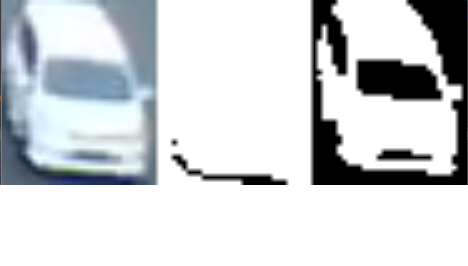
\includegraphics[width=\textwidth]{Images/blackwhite_filter42.PNG}
%\vspace{1.5em}
\caption{} \label{fig:blackwhite_filter}
\end{subfigure}
\begin{subfigure}[t]{0.3\textwidth}
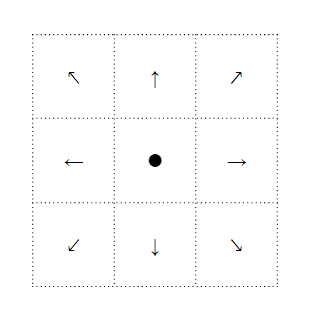
\includegraphics[width=\textwidth]{Images/motion.PNG}
\caption{} \label{fig:motion}
\end{subfigure}
\begin{subfigure}[t]{0.2\textwidth}

\includegraphics[width=\textwidth]{Images/colorspal.png}
%\vspace{0.4em}
\caption{} \label{fig:colorPal}
\end{subfigure}
\caption{(a) Black \& white filter responses, (b) Directional bins, (c) 11 color categories \protect\cite{berlinandkay}} \label{fig:bW_motion}
\end{figure*}

\begin{comment}
 \begin{algorithm}[!h]
  \caption{Achromatic Color}
  \label{algo:achromatic}
  \begin{algorithmic}[1]
  
  \IF{Percentage of White $>$ 25\% \&\& Percentage of Black $<$ 25\%}
	\STATE Color Term = White  	
  \ELSIF {Percentage of Black $>$ 25\% \&\& Percentage of White $<$ 25\%}
  	\STATE Color Term = Black
  \ELSE
  	\STATE Color Term = Gray
  \ENDIF  
  
  \end{algorithmic}
\end{algorithm}
\end{comment}
 
 \begin{algorithm}[!h]
  \caption{Color Term Extraction}
  \label{algo:colorExtract}
  \begin{algorithmic}[1]
    \FOR{Each blob in object}
        \STATE Shrink bounding box (crop image)
        \STATE Create a copy of the cropped image in grayscale
        \STATE Calculate absolute difference between cropped image \& grayscale image
        \STATE Perform threshold on absolute difference to amplify difference
        \STATE Convert results into grayscale \& calculate no. of non-zero pixels
            \IF{Ratio of non-zero pixels $>$ $T_{pivot}$} 
                \STATE Calculate 3D HSV histogram \tab\tab //Chromatic Vehicle
                \STATE Locate maximum bin location of each channel
                \STATE Map the highest bin from each channel to Color Term
            \ELSE 
                \STATE Perform black \& white filter\tab\tab //Achromatic Vehicle
                \STATE Obtain ratio of non-zero pixels from both filters
                \STATE Determine Color Term
            \ENDIF

    \ENDFOR
    \STATE Obtain average dominant color \& return Color Term
  \end{algorithmic}
\end{algorithm}

As for the chromatic colors, we chose to utilize the HSV color space as it is visually more intuitive than the RGB color space. Here, we generated a 3-dimensional HSV histogram with 15 Hue bins, 8 Saturation bins and 8 Value bins. Based on the generated histogram, the maximum value of each bin from all 3 channels is assumed to correspond to the dominant color of the vehicle. However, since the vehicle is moving in the outdoor scene, the ambient and directional lighting (from sun and other light sources) contribute to slight variation of colors. To suit our problem, the dominant color for each frame of a tracked vehicle is averaged out throughout its 
trajectory.
%tracked-lifetime. \ian{is there an illustration of this?  find it hard to imagine it - my lack of image processing background :P}
 
We also note that the achromatic algorithm is an essential step because the 8 Values bins are insufficient to accurately represent vehicles with borderline dominant color as the brightness values may be widely distributed. 
% js: don't quite understand this
%However, should the initial test against the $T_{pivot}$ fails, the proposed method is able to fall back on the HSV histogram results.
 
\paragraph{Color terms.} Next, we addressed \ian{it is just me, but I prefer the word "addressed" than "tackled", just me only} the problem of defining color terms by adopting the eleven common terms in English as described by a study done in 1969 by Berlin and Kay \cite{berlinandkay}. The color categories are white, black, red, green, yellow, blue, brown, purple, pink, orange, and gray. This definition enables us to quantize the range of colors to a fixed number of color categories while taking advantage of the atom-based structure (Refer to Section \ref{SemanticSegmentation}).

\subsubsection{II. Motion information} also plays an important role in the retrieval process as users would often describe the trajectory of a vehicle from a particular incident. 
Instead of generating a 
%high-level understanding 
fine representation of the vehicle's trajectory (conventional motion vectors), 
% verbose... too many of these phrases when it is already understood.
%in our proposed method, 
we %chose to   \js{'chose' is also assumed since it is our method} 
can store a coarser representation of motion information\ian{i think we know what this high-level and low-level but maybe some elaboration for other readers may be good}
in the form of directional categories.
We achieve this by quantizing the extracted motion information of the vehicle trajectories into 9 bins -- 8 directional bins as well as one bin to denote minuscule and negligible motion, as shown in Figure \ref{fig:motion}. The motion vectors are extracted from the centroid of the vehicle, 
with respect to its previous location one second ago; a minimum displacement of 5 pixels determines the presence of motion.
%with a minimal displacement value of 5 pixels from it's previous location 1 second ago.
 
The advantage of such a method is that we are able to fully utilize the atom-based structure (Refer to Section \ref{SemanticSegmentation}) to locate motions of interest in an efficient manner. With this approach, we do not have to consider the various combinations of fine-grained motion trajectories which may occur in realistic outdoor scenes such as carparks. 
%while performing the indexing and retrieval task. 

 \subsection{Semantic Segmentation and Indexing}
 \label{SemanticSegmentation}
 
 \subsubsection{I.\quad Semantic Segmentation}
 
In the proposed method, we adopted the concept of using video cubes or \emph{atoms} from \cite{castanon2016retrieval} as a high-level data structure that frames the data into a spatio-temporal search space.
% js: don't quite understand this line
%to tackle the challenge faced when dealing with a spatio-temporal problem with some variations in the way we implemented them. 
% js: there should be some definition of what an atom is
An atom is defined as a group of cells at a similar spatial location, that spans a certain fixed number of frames; hence forming a spatio-temporal `cube'. Figure \ref{fig:atom} illustrates the atom structure. 
% js: contrast how we use atoms with how Castanon uses it
Contrary to \cite{castanon2016retrieval} which uses these atoms in a tree-like structure that associates each atom with its neighbors as the child nodes, we consider each atom discretely and independently of one another. 
% js: i think this is not necessary to mention
%with an option to co-relate them with information such as source video and vehicle ID

\ian{not sure on print whether that small image is legible, can make it larger?}

\begin{figure*}[!t]
\centering
\begin{subfigure}{0.42\textwidth}
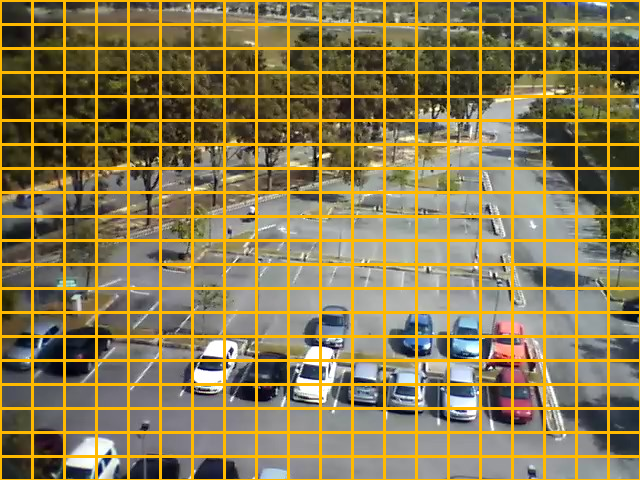
\includegraphics[width=\textwidth]{Images/grids2.png}
\caption{2D Atom Grids} \label{fig:grids}
\end{subfigure}
\begin{subfigure}{0.42\textwidth}
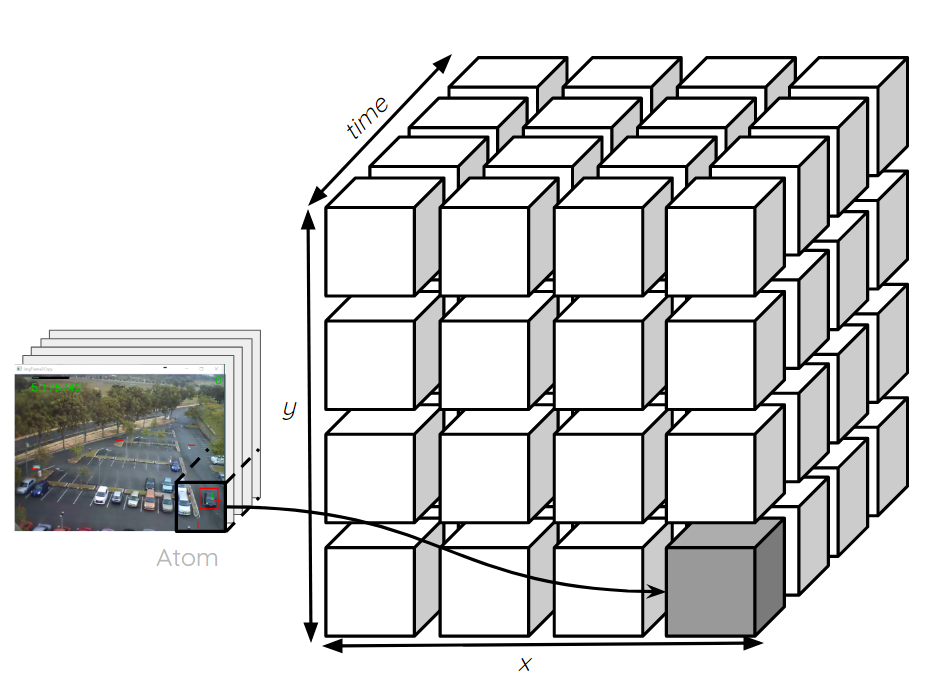
\includegraphics[width=\textwidth]{Images/atom.PNG}
\caption{Atom} \label{fig:atom}
\end{subfigure}
\caption{Atom Structure} \label{fig:atom_struct}
\vspace{-1em}
\end{figure*}
 
Since our video data (see Section \ref{sec:dataset}) has a resolution of 640 $\times$ 480 pixels and frame rate of 10$fps$, we analytically set the dimensions of each atom, $\alpha$ to $\alpha_{width} =32$ pixels, $\alpha_{height} = 24$ pixels and $\alpha_{t} = 10$ frames, which represents the temporal duration of one second. We selected the resolution of the atom ($\alpha_{width},\alpha_{height}$) as such so that the video resolution can be uniformly divide our video into 20 atoms across both its width and height. This approach allows us to distinctly identify each atom from a video by an index $(\alpha_{width},\alpha_{height},\alpha_{t})$ (see Figure \ref{fig:atom_struct}). Similarly, we can store specific occurrences of each semantic type (color, motion) with the same atom index. Though a vehicle blob may be encapsulated by several neighboring atoms, only the atom which corresponds to the centroid of the blob is stored. This is done with the consideration that 
%when a retrieval task is requested,
% js: change this sentence
%the exact bounding box holds lesser weight compared to a precisely retrieved video snippet.  
the precise bounding box location is not essential for retrieving video shots.
 
 \subsubsection{II.\quad Semantic Indexing} 
In order to index the extracted data, we borrowed the idea similar to that of Locality-sensitive Hashing (LSH) used in \cite{castanon2016retrieval} by grouping similar semantics together for quicker retrieval. Our proposed method espouses this by creating unique database tables for each of the 20 semantics (11 colors and 9 motion bins) with the source video, vehicle ID along with the individual atom indices as columns for each table. This allows us to rapidly locate specific atoms with the queried semantic without going through the entire database, as illustrated in Figure \ref{fig:typesofQuery}. The atom structure enables us to make queries based on a specific region of interest, or time slice.

% not relevant to say
%We believe that this method could potentially improve the execution time required for each query, however, we have yet to fully test its efficiency against the normal approach of storing high level information as we have yet to collect a significantly large amount of data to prove this concept.

\ian{love this Figure 5 :-)  Could not have imagine it any better}

 \begin{figure*}[t!]
\centering
\begin{subfigure}{0.25\textwidth}
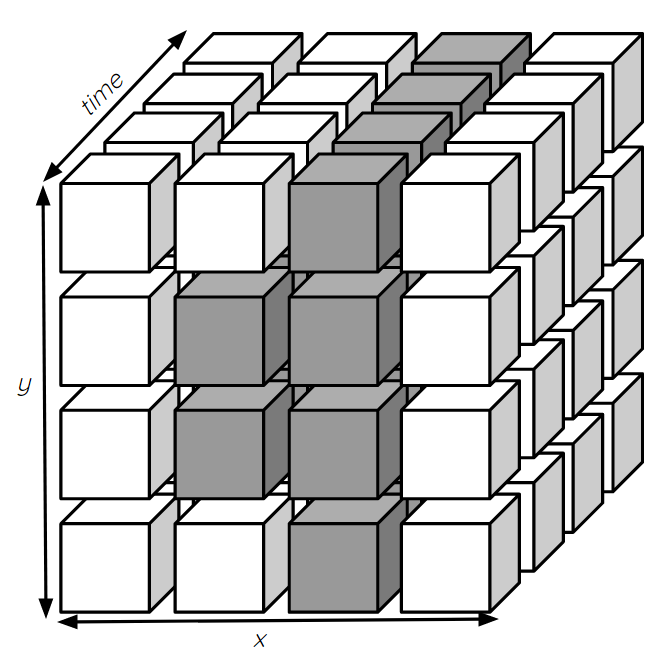
\includegraphics[width=\linewidth]{Images/atom_ROI.PNG}
\caption{Region of Interest} \label{fig:ROI}
\end{subfigure}
%\hspace*{\fill} 
\begin{subfigure}{0.25\textwidth}
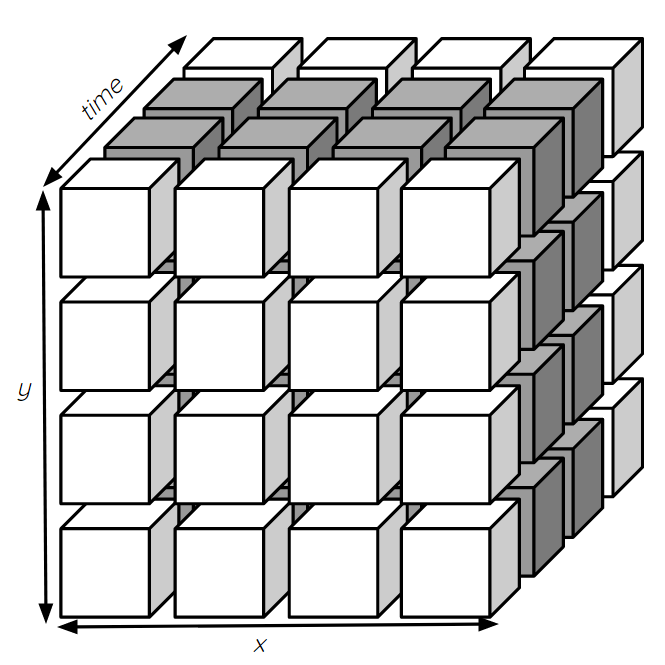
\includegraphics[width=\linewidth]{Images/atom_time_slicing.PNG}
\caption{Time Slicing} \label{fig:timeslicing}
\end{subfigure}
%\hspace*{\fill} 
\vspace{-0.5em}
\caption{Types of Queries} \label{fig:typesofQuery}
\vspace{-0.75em}
\end{figure*}
 
\subsection{Semantic Retrieval}
  
When a color query $\mathbb{C}$ is issued, all vehicles with matching colors are returned.
When a trajectory query $\mathbb{Q}$ is issued, the possible atoms that are matched will be retrieved in temporal order. These retrieved atoms need to be merged to build video shots that will be returned.
%proposed method will extract all possible atoms which satisfies these queries. 
% js: correlated?
%These atoms are then filtered, grouped and correlated based on $atom_t$, vehicle ID as well as the source video. 
% formalizing atom merging
Assume $\mathbb{A}=\{\alpha_{n},\alpha_{n+1},\ldots,\alpha_{N}\}$ is a time-ordered set of retrieved atoms, we intend to piece together relevant atoms to build video shots $\mathbb{S}_i$. This is achieved by performing atom merging if the following condition is met:
\begin{equation}
    \tab\alpha_{n+1} \subset \mathbb{S}_{i} \qquad \textbf{if}\quad t_{\alpha_{n+1}}-t_{\alpha_{n}} < (5*f) 
	\label{formula:atom_merge}
\end{equation}
where $f$ is the video frame rate.
% rewritten as above
%In our setup, an assumption was made that an atom $\alpha_{t}$ is a subset of $\alpha_{t+1}$ if neighboring $\alpha_{t}$'s value is less than 5 seconds apart: \ian{the atoms are technically 1 second apart right?  This is just a curiousity question, will pop into the lab and ask sometime} \cc{yeap, they are technically 1 second apart, however, sometimes the vehicle may be stalled by other vehicles, also, i set 5 secs as i can draw disjointed queries (which is not disccussed here)}

%In the proposed method, %we introduced an approach which allow 
We also introduce a Confidence Value (CV) which sets the sensitivity level of accepting a video shot as among the retrieved results.
%users are able to set the Confidence Value (CV) with a range of 70\% -- 100\% which returns a group of results if it satisfies Equation \ref{formula:satisfyCV}. 
For each shot, we accept each retrieved shot $\mathbb{S}_i$ if it fulfills the following condition:
\begin{equation}
	CV < \frac{\text{length}(\mathbb{S}_i)}{\text{length}(\mathbb{Q})} \times 100\% 
	\label{formula:searchCV}
\end{equation}
This provides a margin of error when performing the query which acts as a trade-off function. 
A lower CV results in returning a larger set of results but at the expense of an increase in retrieved shots, and vice versa. 
%hence returning a larger set of results when the CV is lowered, however while this allows an increase of retrieved data, the overall precision may drop as well.


%Since it is intuitive for users to describe a trajectory by drawing it, 
\paragraph{Search Interface.} The proposed methods were realized in a form of a search interface, which was designed to allow users to construct a query by tracing the trajectory and selecting colors which fit their intended vehicle description. Figure \ref{fig:gui} shows the interface, with the green lines showing the user-selected trajectory query. The underlying atom-based structure allows queries to be formed in a way which emulates the semantics extraction process, eliminating the need for query parsing.
% x
%which in turn reduces the need of preprocessing and post-processing any of the query. However, the current implementation of the proposed method search interface has yet to include time slicing query options. 
\begin{figure*}[t!]
\centering
\begin{subfigure}{0.48\textwidth}
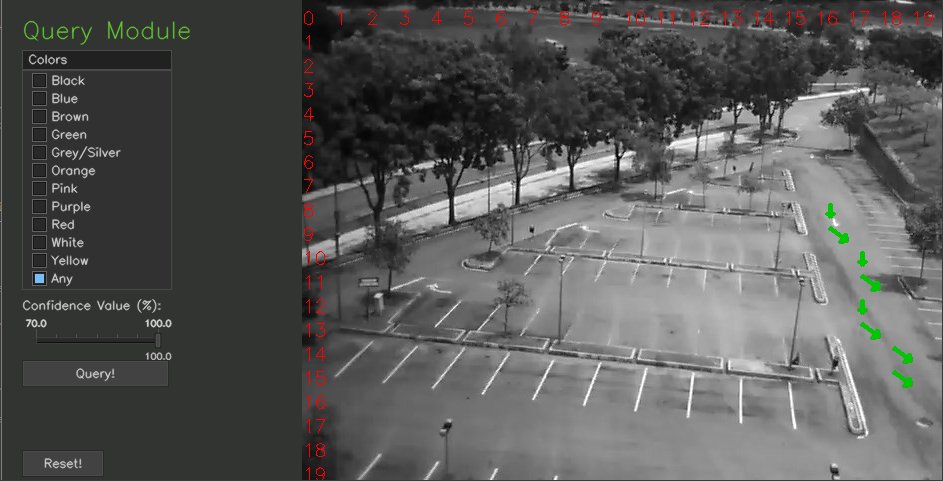
\includegraphics[width=\linewidth]{Images/test1-8inputs.PNG}
\caption{Motion Test Case 1 (TQ1)} \label{fig:test1}
\end{subfigure}
%\hspace*{\fill} 
\begin{subfigure}{0.48\textwidth}
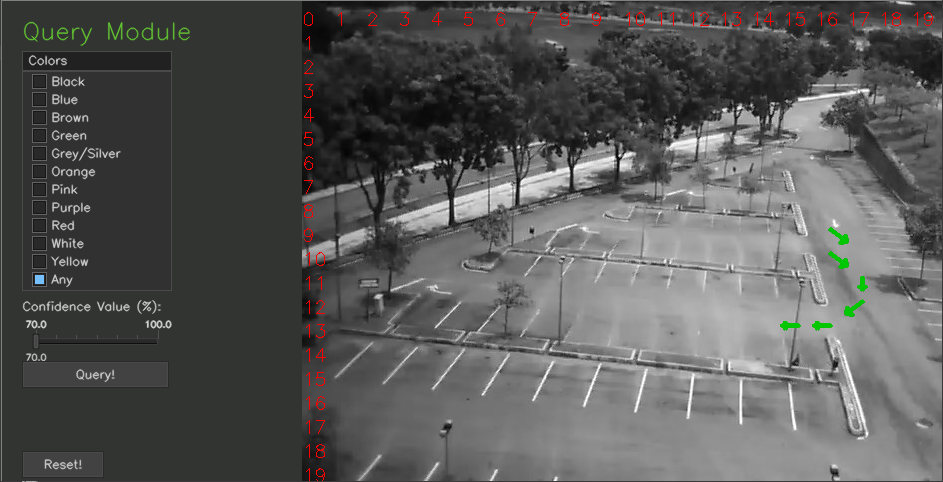
\includegraphics[width=\linewidth]{Images/test2-6input.PNG}
\caption{Motion Test Case 2 (TQ2)} \label{fig:test2}
\end{subfigure}
%\hspace*{\fill} 
\vspace{-0.5em}
\caption{Search interface for the proposed framework} \label{fig:gui}
\vspace{-1em}
\end{figure*}



%\paragraph{Notes and Comments.}
%The current implementation of the proposed method search interface has yet to include time slicing query options.

 \section{Experiments}

 \subsection{Dataset}
 \label{sec:dataset}
This section describes the video data used in the development and evaluation of the proposed method. We collected a new video dataset consisting of videos recorded from a university's outdoor carpark area over a duration of several months. A single stationary camera was set up 
%in one of the laboratories 
to record the video on weekdays throughout the week from 8:30AM to 6:30PM.
% I think we can save the reader from these details. Unless we are releasing our data, then it makes sense to inform how it was recorded.
%The camera was configured to record 6-minute videos for ease of access and processing. Hence, a total of 100 videos were captured for a single day. 
These videos were recorded in a compressed H.264 MPEG-4 format with a resolution of 640 $\times$ 480 pixels and frame rate of 10$fps$.  %However, due to some unforeseen glitches during the video capture, it is noted that some of the days does not contain the full 10 hours worth of videos. 
Figure \ref{fig:challenges}a shows a wide range of challenges found in the recorded video data: severe morning and afternoon shadows, rainy weather, and reflections. Due to the scale of experiment, we selected 2 days of video data (totaling 20 hours)
%- 18th \& 19th October 2016) 
for the work in this paper.

\begin{comment}
\begin{figure*}

    \centering
    \begin{subfigure}[b]{0.23\textwidth}
        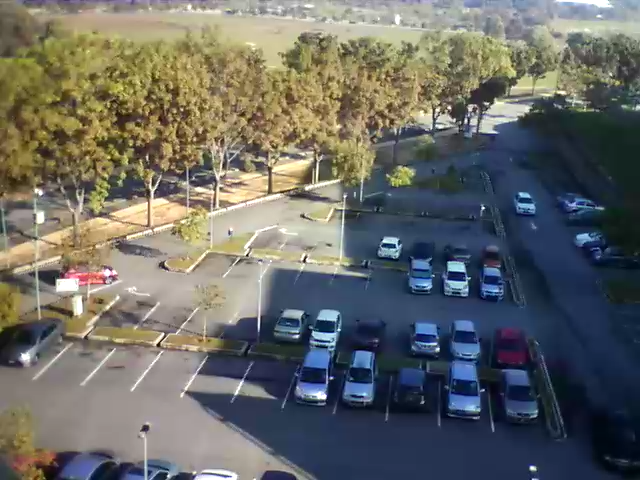
\includegraphics[width=\textwidth]{Images/shadow.png}
        \caption{Severe shadow casted on the carpark (08:48AM)}
        \label{fig:shadow1}
        
    \end{subfigure}
    ~ %add desired spacing between images, e. g. ~, \quad, \qquad, \hfill etc. 
      %(or a blank line to force the subfigure onto a new line)
    \begin{subfigure}[b]{0.23\textwidth}
        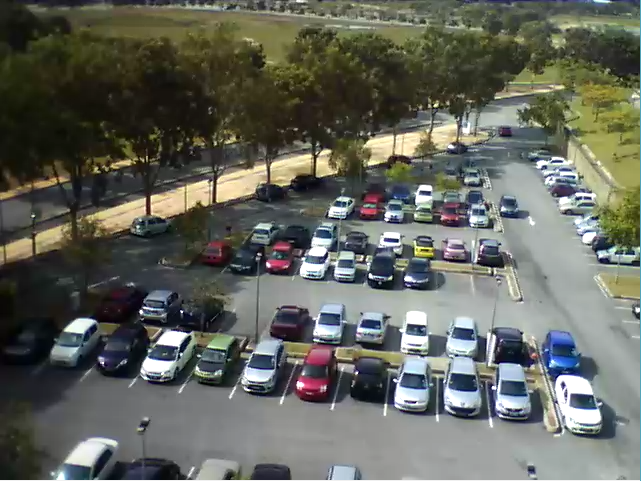
\includegraphics[width=\textwidth]{Images/shadow2.png}
        \caption{Severe shadow casted on the carpark (04:06PM)}
        \label{fig:shadow2}
    \end{subfigure}
    ~ %add desired spacing between images, e. g. ~, \quad, \qquad, \hfill etc. 
    %(or a blank line to force the subfigure onto a new line)
    \begin{subfigure}[b]{0.23\textwidth}
 
        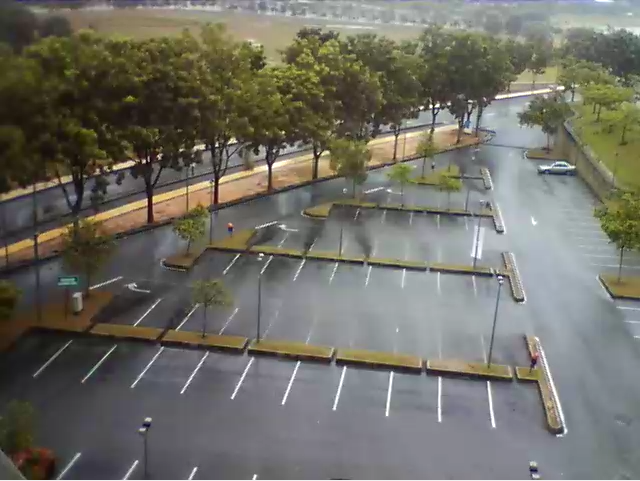
\includegraphics[width=\textwidth]{Images/rain.png}
        \caption{Rainy day - reflective surface affecting overall color }
        \label{fig:rainyday}
    \end{subfigure}
     ~ %add desired spacing between images, e. g. ~, \quad, \qquad, \hfill etc. 
    %(or a blank line to force the subfigure onto a new line)
    \begin{subfigure}[b]{0.23\textwidth}
        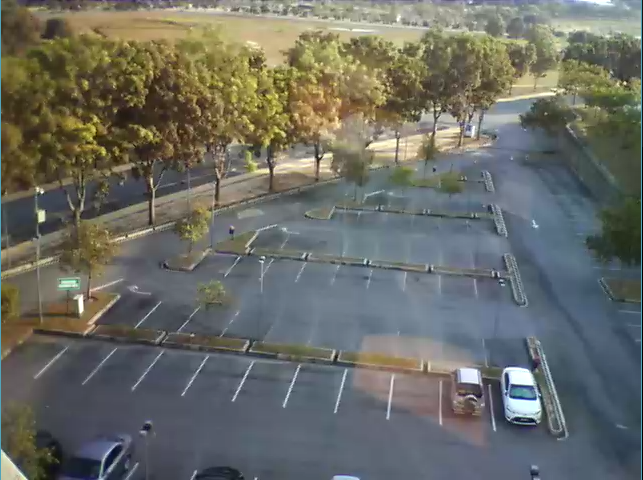
\includegraphics[width=\textwidth]{Images/reflection.png}
        \caption{Reflection from within the laboratory (lower right)}
        \label{fig:reflection}
    \end{subfigure}
    \caption{Challenges encountered in the recorded video data}\label{fig:challenges}
    
\end{figure*}
\end{comment}


\begin{figure*}
    \centering
    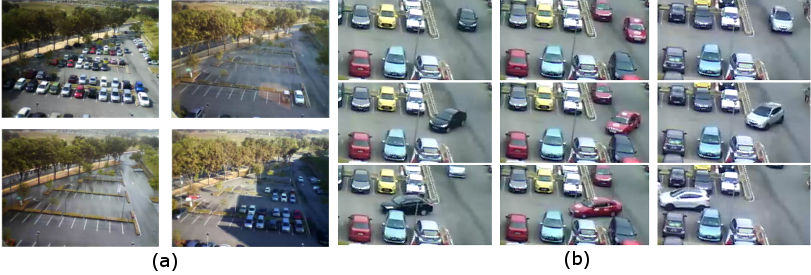
\includegraphics[width=\textwidth]{Images/sceneNresult.PNG}
    \caption{(a) Various carpark scene challenges throughout the day (severe shadow, weather condition and reflections)  (b) Sample screenshots of 3 retrieved shots (left, center, right columns) for query TQ2 (turning into junction)}
    \vspace{-1em}
    \label{fig:challenges}
    %\vspace{-0.5em}
\end{figure*}

\subsection{Experiment Methodology}

To validate our method for vehicle color and motion retrieval, the ground truth states were manually labeled by a few annotators and cross-checked to arrive at a consensus. This allows us to validate the efficacy of our proposed automated method against human observations.
Our system was implemented on an Intel i7 machine with 16GB RAM, GeForce GTX 1060 GPU.
% remove to prevent more questions about the fps here
%The entire process pipeline (including additional overhead for writing to the database), from start to end, averaged at around 11$fps$. 
In order to\ian{remove "have to"} analyze both color and motion semantics individually 
%semantic extraction components (i. color \& ii. motion), %we chose to disassociate%
they are evaluated separately to measure their individual performances. 

\subsubsection{Color Retrieval} \tab

To measure the performance of the color retrieval module, we follow through the pipeline by extracting unique objects from each of the 11 color tables. 
%regardless of the motion information. 
The retrieved results are then compared against the ground truth. The ground truth distribution of vehicle colors is shown in Table \ref{table:colorDist}.

\vspace{-0.5em}
\begin{table}[t!]
	\centering
	\caption{Ground truth distribution vehicle colors ordered by occurrence}
    \label{table:colorDist}
	\begin{tabular}{lccccccccccc}
		\toprule
			Color\quad & Gray & Black & White & Red & Blue & Orange & Yellow & Green & Pink & Purple & Brown \\
		\midrule
        \# & 365 & 182 & 150 & 60 & 19 & 15 & 13 & 10 & 9 & 7 & 7 \\
        \% & 43.6 & 21.7 & 17.9 & 7.2 & 2.3 & 1.8 & 1.6 & 1.2 & 1.1 & 0.8 & 0.8 \\
%        	Gray    & \tab 365  & 43.61 \\
% 			Black   & \tab 182  & 21.74 \\ 
% 			White   & \tab 150  & 17.92 \\
% 			Red     & \tab 60   & 7.17 \\
% 			Blue    & \tab 19   & 2.27 \\ 
% 			Orange  & \tab 15   & 1.79 \\ 
% 			Yellow  & \tab 13   & 1.55 \\ 
% 			Green   & \tab 10   & 1.19 \\ 
% 			Pink    & \tab 9    & 1.08 \\
% 			Purple  & \tab 7    & 0.84 \\
% 			Brown   & \tab 7    & 0.84 \\
		\bottomrule
	\end{tabular}
    \vspace{-1em}
\end{table}

\subsubsection{Motion Retrieval} \tab

We specified 2 specific motion paths or trajectory queries (TQ) that we intend to validate: TQ1) Heading southward (see Fig. \ref{fig:test1}) \& TQ2) Turning in a junction (see Fig. \ref{fig:test2}). The distribution of these test cases are 252 (86.3\%) and 40 (13.7 \%) trajectories for TQ1 and TQ2 respectively. \ian{this may be too few for testing - also, hard to see from the images}

To measure the performance of the motion retrieval method, we performed evaluation on both TQ1 and TQ2 without consideration for the vehicle color. These experiments were tested on a few CV values (70\%, 80\%, 90\%) and different
% js: why reducing?
%while reducing the 
number of atom query inputs to test the impact of trajectory details.
%detailed trajectory against a general trajectory direction.

\subsubsection{Evaluation metrics:} We used 3 evaluation metrics - Precision, Recall as well as the $F_1$ score to determine the overall performance of the system. Correct matches will be regarded as true positives, $tp$. False positives, $fp$ is the total number of retrieved results minus the true positives, while false negatives, $fn$ is the total number of correct results minus true positives. Precision, Recall and $F_{1}$ score is computed as:
\begin{center}
\begin{equation}
\text{Precision}  = \frac{tp}{tp + fp}  \text{ ; }
\text{Recall}  = \frac{tp}{tp + fn} \text{ ; }
\text{F1-score}  = 2\cdot\frac{\text{Precision} \cdot \text{Recall}}{\text{Precision} + \text{Recall}}
\vspace{-0.5em}
\end{equation}
\end{center}

%\noindent where $tp$ is the true positives, $fp$ is the false positives and $fn$ is the false negatives.


\begin{comment}
The Accuracy metric was not used for measuring the overall performance of the detection task as the data is severely imbalanced and this metric may be bias towards the activities with larger number of occurrences (see Table~\ref{table:GroundTruth}), i.e. the `Enter' and `Exit' activities are around 9 times more than the rest. Instead, the F1-score was used as it is the harmonic mean of the Precision and Recall scores.  
\end{comment}


\subsection{Experiment Results and Discussion}
The performance of the proposed method is computed by comparing the annotated ground truth against the retrieved results. %Color semantics retrieval is done regardless of the motion path while motion semantics are retrieved based on the test cases regardless of the color information.

\subsubsection{Color Retrieval} \tab

Table \ref{table:colorMatrix} reports the confusion matrix of the color retrieval task. 
%While most of the color terms were extracted correctly \ian{this is not true, e.g. Black retrieved as Gray is 48 ... btw, is the word "predicted color" the correct term?  "deduced"?}, 
The overall precision stands at 54\%, with a recall of 36\% and $F_1$ score of 39\%. The cells in Table \ref{table:colorMatrix} marked in green indicate the highest count of correctly predicted colors, while the cells marked in red indicate the highest count of incorrect predictions for each color. Our method is able to predict correctly a majority of cases for seven out of eleven colors.

Based on the obtained results, we learn that the $T_{pivot}$ needs to be adjusted as too many chromatic vehicles were classified as achromatic vehicles which in turned affected the overall performance of the proposed method. We hypothesize that better results can be obtained by careful adjustment of $T_{pivot}$ or attempt to learn a suitable color model as in \cite{hu2015vehicle,rachmadi2015vehicle} for this particular scene. We observe that vehicles with lighter and darker shades were particularly difficult as they do not contain enough chromatic hues to arrive at a correct prediction.  

While the classification of achromatic versus chromatic vehicles faced considerable difficulties, the black \& white filters provide a considerably good result when determining the different categories of achromatic vehicles which may be useful for processing in grayscale. Based on our observation, most errors usually occur when the vehicles are in locations where the intensity of shadows overpowered the lighter-shade vehicles in terms of coverage area. 

\begin{table}[]
\centering
\caption{Confusion matrix for color retrieval task}
\vspace{1.5em}
\label{table:colorMatrix}
\resizebox{\columnwidth}{!}{
\begin{tabular}{ccccccccccccc}
\cline{3-13}
                                                      & \multicolumn{1}{l|}{}          & \multicolumn{11}{c|}{Predicted Color}                                                                                                                                                                                                                                                                                                                                                                                                                                                                                                                                                                                                                             \\ \cline{3-13} 
                                                      & \multicolumn{1}{c|}{}          & \multicolumn{1}{c|}{Gray}                                 & \multicolumn{1}{c|}{Black}                                & \multicolumn{1}{c|}{White}                                & \multicolumn{1}{c|}{Red}                                & \multicolumn{1}{c|}{Blue}                               & \multicolumn{1}{c|}{Orange}                             & \multicolumn{1}{c|}{Yellow}                             & \multicolumn{1}{c|}{Green}                              & \multicolumn{1}{c|}{Pink}                               & \multicolumn{1}{c|}{Purple}                             & \multicolumn{1}{c|}{Brown}                              \\ \hline
\multicolumn{1}{|l|}{}                                & \multicolumn{1}{c|}{Gray}      & \multicolumn{1}{c|}{\cellcolor[HTML]{32CB00}\textbf{236}} & \multicolumn{1}{c|}{61}                                   & \multicolumn{1}{c|}{68}                                   & \multicolumn{1}{c|}{0}                                  & \multicolumn{1}{c|}{0}                                  & \multicolumn{1}{c|}{0}                                  & \multicolumn{1}{c|}{0}                                  & \multicolumn{1}{c|}{0}                                  & \multicolumn{1}{c|}{0}                                  & \multicolumn{1}{c|}{0}                                  & \multicolumn{1}{c|}{0}                                  \\ \cline{2-13} 
\multicolumn{1}{|l|}{}                                & \multicolumn{1}{c|}{Black}     & \multicolumn{1}{c|}{48}                                   & \multicolumn{1}{c|}{\cellcolor[HTML]{32CB00}\textbf{134}} & \multicolumn{1}{c|}{0}                                    & \multicolumn{1}{c|}{0}                                  & \multicolumn{1}{c|}{0}                                  & \multicolumn{1}{c|}{0}                                  & \multicolumn{1}{c|}{0}                                  & \multicolumn{1}{c|}{0}                                  & \multicolumn{1}{c|}{0}                                  & \multicolumn{1}{c|}{0}                                  & \multicolumn{1}{c|}{0}                                  \\ \cline{2-13} 
\multicolumn{1}{|l|}{}                                & \multicolumn{1}{c|}{White}     & \multicolumn{1}{c|}{26}                                   & \multicolumn{1}{c|}{4}                                    & \multicolumn{1}{c|}{\cellcolor[HTML]{32CB00}\textbf{120}} & \multicolumn{1}{c|}{0}                                  & \multicolumn{1}{c|}{0}                                  & \multicolumn{1}{c|}{0}                                  & \multicolumn{1}{c|}{0}                                  & \multicolumn{1}{c|}{0}                                  & \multicolumn{1}{c|}{0}                                  & \multicolumn{1}{c|}{0}                                  & \multicolumn{1}{c|}{0}                                  \\ \cline{2-13} 
\multicolumn{1}{|l|}{}                                & \multicolumn{1}{c|}{Red}       & \multicolumn{1}{c|}{27}                                   & \multicolumn{1}{c|}{25}                                   & \multicolumn{1}{c|}{0}                                    & \multicolumn{1}{c|}{2}                                  & \multicolumn{1}{c|}{0}                                  & \multicolumn{1}{c|}{0}                                  & \multicolumn{1}{c|}{0}                                  & \multicolumn{1}{c|}{0}                                  & \multicolumn{1}{c|}{4}                                  & \multicolumn{1}{c|}{\cellcolor[HTML]{FE0000}\textbf{2}} & \multicolumn{1}{c|}{0}                                  \\ \cline{2-13} 
\multicolumn{1}{|l|}{}                                & \multicolumn{1}{c|}{Blue}      & \multicolumn{1}{c|}{3}                                    & \multicolumn{1}{c|}{10}                                   & \multicolumn{1}{c|}{0}                                    & \multicolumn{1}{c|}{0}                                  & \multicolumn{1}{c|}{\cellcolor[HTML]{32CB00}\textbf{6}} & \multicolumn{1}{c|}{0}                                  & \multicolumn{1}{c|}{0}                                  & \multicolumn{1}{c|}{0}                                  & \multicolumn{1}{c|}{0}                                  & \multicolumn{1}{c|}{0}                                  & \multicolumn{1}{c|}{0}                                  \\ \cline{2-13} 
\multicolumn{1}{|l|}{}                                & \multicolumn{1}{c|}{Orange}    & \multicolumn{1}{c|}{8}                                    & \multicolumn{1}{c|}{3}                                    & \multicolumn{1}{c|}{0}                                    & \multicolumn{1}{c|}{0}                                  & \multicolumn{1}{c|}{0}                                  & \multicolumn{1}{c|}{\cellcolor[HTML]{32CB00}\textbf{3}} & \multicolumn{1}{c|}{0}                                  & \multicolumn{1}{c|}{0}                                  & \multicolumn{1}{c|}{0}                                  & \multicolumn{1}{c|}{1}                                  & \multicolumn{1}{c|}{0}                                  \\ \cline{2-13} 
\multicolumn{1}{|l|}{}                                & \multicolumn{1}{c|}{Yellow}    & \multicolumn{1}{c|}{3}                                    & \multicolumn{1}{c|}{1}                                    & \multicolumn{1}{c|}{2}                                    & \multicolumn{1}{c|}{0}                                  & \multicolumn{1}{c|}{0}                                  & \multicolumn{1}{c|}{0}                                  & \multicolumn{1}{c|}{\cellcolor[HTML]{32CB00}\textbf{7}} & \multicolumn{1}{c|}{0}                                  & \multicolumn{1}{c|}{0}                                  & \multicolumn{1}{c|}{0}                                  & \multicolumn{1}{c|}{0}                                  \\ \cline{2-13} 
\multicolumn{1}{|l|}{}                                & \multicolumn{1}{c|}{Green}     & \multicolumn{1}{c|}{5}                                    & \multicolumn{1}{c|}{1}                                    & \multicolumn{1}{c|}{4}                                    & \multicolumn{1}{c|}{0}                                  & \multicolumn{1}{c|}{0}                                  & \multicolumn{1}{c|}{0}                                  & \multicolumn{1}{c|}{0}                                  & \multicolumn{1}{c|}{\cellcolor[HTML]{C0C0C0}\textbf{0}} & \multicolumn{1}{c|}{0}                                  & \multicolumn{1}{c|}{0}                                  & \multicolumn{1}{c|}{0}                                  \\ \cline{2-13} 
\multicolumn{1}{|l|}{}                                & \multicolumn{1}{c|}{Pink}      & \multicolumn{1}{c|}{1}                                    & \multicolumn{1}{c|}{0}                                    & \multicolumn{1}{c|}{0}                                    & \multicolumn{1}{c|}{\cellcolor[HTML]{FE0000}\textbf{3}} & \multicolumn{1}{c|}{0}                                  & \multicolumn{1}{c|}{0}                                  & \multicolumn{1}{c|}{0}                                  & \multicolumn{1}{c|}{0}                                  & \multicolumn{1}{c|}{\cellcolor[HTML]{32CB00}\textbf{5}} & \multicolumn{1}{c|}{0}                                  & \multicolumn{1}{c|}{0}                                  \\ \cline{2-13} 
\multicolumn{1}{|l|}{}                                & \multicolumn{1}{c|}{Purple}    & \multicolumn{1}{c|}{3}                                    & \multicolumn{1}{c|}{3}                                    & \multicolumn{1}{c|}{0}                                    & \multicolumn{1}{c|}{0}                                  & \multicolumn{1}{c|}{0}                                  & \multicolumn{1}{c|}{0}                                  & \multicolumn{1}{c|}{0}                                  & \multicolumn{1}{c|}{0}                                  & \multicolumn{1}{c|}{0}                                  & \multicolumn{1}{c|}{1}                                  & \multicolumn{1}{c|}{0}                                  \\ \cline{2-13} 
\multicolumn{1}{|l|}{\multirow{-11}{*}{\rotatebox[origin=c]{90}{Actual Color}}} & \multicolumn{1}{c|}{Brown}     & \multicolumn{1}{c|}{3}                                    & \multicolumn{1}{c|}{4}                                    & \multicolumn{1}{c|}{0}                                    & \multicolumn{1}{c|}{0}                                  & \multicolumn{1}{c|}{0}                                  & \multicolumn{1}{c|}{0}                                  & \multicolumn{1}{c|}{0}                                  & \multicolumn{1}{c|}{0}                                  & \multicolumn{1}{c|}{0}                                  & \multicolumn{1}{c|}{0}                                  & \multicolumn{1}{c|}{\cellcolor[HTML]{C0C0C0}\textbf{0}} \\ \hline
                                                      & \multicolumn{1}{l}{}           & \multicolumn{1}{l}{}                                      & \multicolumn{1}{l}{}                                      & \multicolumn{1}{l}{}                                      & \multicolumn{1}{l}{}                                    & \multicolumn{1}{l}{}                                    & \multicolumn{1}{l}{}                                    & \multicolumn{1}{l}{}                                    & \multicolumn{1}{l}{}                                    & \multicolumn{1}{l}{}                                    & \multicolumn{1}{l}{}                                    & \multicolumn{1}{l}{}                                    \\ \hline
\multicolumn{1}{|l|}{}                                & \multicolumn{1}{c|}{Precision} & \multicolumn{1}{c|}{65.01}                                & \multicolumn{1}{c|}{54.47}                                & \multicolumn{1}{c|}{61.86}                                & \multicolumn{1}{c|}{40.00}                              & \multicolumn{1}{c|}{100.00}                             & \multicolumn{1}{c|}{100.00}                             & \multicolumn{1}{c|}{100.00}                             & \multicolumn{1}{c|}{N/A}                                & \multicolumn{1}{c|}{55.56}                              & \multicolumn{1}{c|}{25.00}                              & \multicolumn{1}{c|}{N/A}                                \\ \cline{2-13} 
\multicolumn{1}{|l|}{}                                & \multicolumn{1}{c|}{Recall}    & \multicolumn{1}{c|}{64.66}                                & \multicolumn{1}{c|}{73.63}                                & \multicolumn{1}{c|}{80.00}                                & \multicolumn{1}{c|}{3.33}                               & \multicolumn{1}{c|}{31.58}                              & \multicolumn{1}{c|}{20.00}                              & \multicolumn{1}{c|}{53.85}                              & \multicolumn{1}{c|}{0.00}                               & \multicolumn{1}{c|}{55.56}                              & \multicolumn{1}{c|}{14.29}                              & \multicolumn{1}{c|}{0.00}                               \\ \cline{2-13} 
\multicolumn{1}{|l|}{\multirow{-3}{*}{\rotatebox[origin=c]{90}{Result}}}        & \multicolumn{1}{c|}{F1 Score}  & \multicolumn{1}{c|}{64.84}                                & \multicolumn{1}{c|}{62.62}                                & \multicolumn{1}{c|}{69.77}                                & \multicolumn{1}{c|}{6.15}                               & \multicolumn{1}{c|}{48.00}                              & \multicolumn{1}{c|}{33.33}                              & \multicolumn{1}{c|}{70.00}                              & \multicolumn{1}{c|}{N/A}                                & \multicolumn{1}{c|}{55.56}                              & \multicolumn{1}{c|}{18.18}                              & \multicolumn{1}{c|}{N/A}                                \\ \hline
\end{tabular}%
}
\end{table}


\begin{comment}
%% This table does not have the predicted & actual label
% Please add the following required packages to your document preamble:
% \usepackage[table,xcdraw]{xcolor}
% If you use beamer only pass "xcolor=table" option, i.e. \documentclass[xcolor=table]{beamer}
\begin{table}[]
\centering
\caption{My caption}
\label{my-label}
\begin{tabular}{cccccccccccc}
\cline{2-12}
\multicolumn{1}{c|}{} & \multicolumn{1}{c|}{Gray} & \multicolumn{1}{c|}{Black} & \multicolumn{1}{c|}{White} & \multicolumn{1}{c|}{Red} & \multicolumn{1}{c|}{Blue} & \multicolumn{1}{c|}{Orange} & \multicolumn{1}{c|}{Yellow} & \multicolumn{1}{c|}{Green} & \multicolumn{1}{c|}{Pink} & \multicolumn{1}{c|}{Purple} & \multicolumn{1}{c|}{Brown} \\ \hline
\multicolumn{1}{|c|}{Gray} & \multicolumn{1}{c|}{\cellcolor[HTML]{32CB00}\textbf{236}} & \multicolumn{1}{c|}{61} & \multicolumn{1}{c|}{68} & \multicolumn{1}{c|}{0} & \multicolumn{1}{c|}{0} & \multicolumn{1}{c|}{0} & \multicolumn{1}{c|}{0} & \multicolumn{1}{c|}{0} & \multicolumn{1}{c|}{0} & \multicolumn{1}{c|}{0} & \multicolumn{1}{c|}{0} \\ \hline
\multicolumn{1}{|c|}{Black} & \multicolumn{1}{c|}{48} & \multicolumn{1}{c|}{\cellcolor[HTML]{32CB00}\textbf{134}} & \multicolumn{1}{c|}{0} & \multicolumn{1}{c|}{0} & \multicolumn{1}{c|}{0} & \multicolumn{1}{c|}{0} & \multicolumn{1}{c|}{0} & \multicolumn{1}{c|}{0} & \multicolumn{1}{c|}{0} & \multicolumn{1}{c|}{0} & \multicolumn{1}{c|}{0} \\ \hline
\multicolumn{1}{|c|}{White} & \multicolumn{1}{c|}{26} & \multicolumn{1}{c|}{4} & \multicolumn{1}{c|}{\cellcolor[HTML]{32CB00}\textbf{120}} & \multicolumn{1}{c|}{0} & \multicolumn{1}{c|}{0} & \multicolumn{1}{c|}{0} & \multicolumn{1}{c|}{0} & \multicolumn{1}{c|}{0} & \multicolumn{1}{c|}{0} & \multicolumn{1}{c|}{0} & \multicolumn{1}{c|}{0} \\ \hline
\multicolumn{1}{|c|}{Red} & \multicolumn{1}{c|}{27} & \multicolumn{1}{c|}{25} & \multicolumn{1}{c|}{0} & \multicolumn{1}{c|}{2} & \multicolumn{1}{c|}{0} & \multicolumn{1}{c|}{0} & \multicolumn{1}{c|}{0} & \multicolumn{1}{c|}{0} & \multicolumn{1}{c|}{4} & \multicolumn{1}{c|}{\cellcolor[HTML]{FE0000}\textbf{2}} & \multicolumn{1}{c|}{0} \\ \hline
\multicolumn{1}{|c|}{Blue} & \multicolumn{1}{c|}{3} & \multicolumn{1}{c|}{10} & \multicolumn{1}{c|}{0} & \multicolumn{1}{c|}{0} & \multicolumn{1}{c|}{\cellcolor[HTML]{32CB00}\textbf{6}} & \multicolumn{1}{c|}{0} & \multicolumn{1}{c|}{0} & \multicolumn{1}{c|}{0} & \multicolumn{1}{c|}{0} & \multicolumn{1}{c|}{0} & \multicolumn{1}{c|}{0} \\ \hline
\multicolumn{1}{|c|}{Orange} & \multicolumn{1}{c|}{8} & \multicolumn{1}{c|}{3} & \multicolumn{1}{c|}{0} & \multicolumn{1}{c|}{0} & \multicolumn{1}{c|}{0} & \multicolumn{1}{c|}{\cellcolor[HTML]{32CB00}\textbf{3}} & \multicolumn{1}{c|}{0} & \multicolumn{1}{c|}{0} & \multicolumn{1}{c|}{0} & \multicolumn{1}{c|}{1} & \multicolumn{1}{c|}{0} \\ \hline
\multicolumn{1}{|c|}{Yellow} & \multicolumn{1}{c|}{3} & \multicolumn{1}{c|}{1} & \multicolumn{1}{c|}{2} & \multicolumn{1}{c|}{0} & \multicolumn{1}{c|}{0} & \multicolumn{1}{c|}{0} & \multicolumn{1}{c|}{\cellcolor[HTML]{32CB00}\textbf{7}} & \multicolumn{1}{c|}{0} & \multicolumn{1}{c|}{0} & \multicolumn{1}{c|}{0} & \multicolumn{1}{c|}{0} \\ \hline
\multicolumn{1}{|c|}{Green} & \multicolumn{1}{c|}{5} & \multicolumn{1}{c|}{1} & \multicolumn{1}{c|}{4} & \multicolumn{1}{c|}{0} & \multicolumn{1}{c|}{0} & \multicolumn{1}{c|}{0} & \multicolumn{1}{c|}{0} & \multicolumn{1}{c|}{\cellcolor[HTML]{C0C0C0}\textbf{0}} & \multicolumn{1}{c|}{0} & \multicolumn{1}{c|}{0} & \multicolumn{1}{c|}{0} \\ \hline
\multicolumn{1}{|c|}{Pink} & \multicolumn{1}{c|}{1} & \multicolumn{1}{c|}{0} & \multicolumn{1}{c|}{0} & \multicolumn{1}{c|}{\cellcolor[HTML]{FE0000}\textbf{3}} & \multicolumn{1}{c|}{0} & \multicolumn{1}{c|}{0} & \multicolumn{1}{c|}{0} & \multicolumn{1}{c|}{0} & \multicolumn{1}{c|}{\cellcolor[HTML]{32CB00}\textbf{5}} & \multicolumn{1}{c|}{0} & \multicolumn{1}{c|}{0} \\ \hline
\multicolumn{1}{|c|}{Purple} & \multicolumn{1}{c|}{3} & \multicolumn{1}{c|}{3} & \multicolumn{1}{c|}{0} & \multicolumn{1}{c|}{0} & \multicolumn{1}{c|}{0} & \multicolumn{1}{c|}{0} & \multicolumn{1}{c|}{0} & \multicolumn{1}{c|}{0} & \multicolumn{1}{c|}{0} & \multicolumn{1}{c|}{1} & \multicolumn{1}{c|}{0} \\ \hline
\multicolumn{1}{|c|}{Brown} & \multicolumn{1}{c|}{3} & \multicolumn{1}{c|}{4} & \multicolumn{1}{c|}{0} & \multicolumn{1}{c|}{0} & \multicolumn{1}{c|}{0} & \multicolumn{1}{c|}{0} & \multicolumn{1}{c|}{0} & \multicolumn{1}{c|}{0} & \multicolumn{1}{c|}{0} & \multicolumn{1}{c|}{0} & \multicolumn{1}{c|}{\cellcolor[HTML]{C0C0C0}\textbf{0}} \\ \hline
\multicolumn{1}{l}{} & \multicolumn{1}{l}{} & \multicolumn{1}{l}{} & \multicolumn{1}{l}{} & \multicolumn{1}{l}{} & \multicolumn{1}{l}{} & \multicolumn{1}{l}{} & \multicolumn{1}{l}{} & \multicolumn{1}{l}{} & \multicolumn{1}{l}{} & \multicolumn{1}{l}{} & \multicolumn{1}{l}{} \\ \hline
\multicolumn{1}{|c|}{Precision} & \multicolumn{1}{c|}{65.01} & \multicolumn{1}{c|}{54.47} & \multicolumn{1}{c|}{61.86} & \multicolumn{1}{c|}{40.00} & \multicolumn{1}{c|}{100.00} & \multicolumn{1}{c|}{100.00} & \multicolumn{1}{c|}{100.00} & \multicolumn{1}{c|}{N/A} & \multicolumn{1}{c|}{55.56} & \multicolumn{1}{c|}{25.00} & \multicolumn{1}{c|}{N/A} \\ \hline
\multicolumn{1}{|c|}{Recall} & \multicolumn{1}{c|}{64.66} & \multicolumn{1}{c|}{73.63} & \multicolumn{1}{c|}{80.00} & \multicolumn{1}{c|}{3.33} & \multicolumn{1}{c|}{31.58} & \multicolumn{1}{c|}{20.00} & \multicolumn{1}{c|}{53.85} & \multicolumn{1}{c|}{0.00} & \multicolumn{1}{c|}{55.56} & \multicolumn{1}{c|}{14.29} & \multicolumn{1}{c|}{0.00} \\ \hline
\multicolumn{1}{|c|}{F1 Score} & \multicolumn{1}{c|}{64.84} & \multicolumn{1}{c|}{62.62} & \multicolumn{1}{c|}{69.77} & \multicolumn{1}{c|}{6.15} & \multicolumn{1}{c|}{48.00} & \multicolumn{1}{c|}{33.33} & \multicolumn{1}{c|}{70.00} & \multicolumn{1}{c|}{N/A} & \multicolumn{1}{c|}{55.56} & \multicolumn{1}{c|}{18.18} & \multicolumn{1}{c|}{N/A} \\ \hline
\end{tabular}
\end{table}

\end{comment}
\subsubsection{Motion Retrieval} \tab

The retrieved trajectory shots are validated against the annotated ground truth labels to obtain our results. As it is difficult to pinpoint the exact ``scene'' where the test cases occur, we use a time window of $\pm T$ seconds to indicate a range whereby a retrieved motion can be correctly matched to the ground truth label. We fixed $T=5$ in our experiments, similar to that used in the tracking evaluation of \cite{lim2017}. 

\ian{just my thoughts: the above can be elaborated to make it sound more "canggih" as there is a need to compress the time or expand the time of the trajectory etc.}

Table \ref{table:motionResults} shows the results of the motion retrieval task with varying Confidence Values (CV) and varying number of atom inputs in the trajectory query. For TQ1, the total number of atom inputs varied from 5 to 8 inputs while TQ2 is represented by a shorter trajectory of 4 to 6 inputs as it concerns a junction turning query. For TQ1 \& TQ2, the overall average precision is around 89\% \& 50\% while the recall is at 27\% \& 59\% respectively.  Based on the $F_1$ scores, the results show that the proposed retrieval method works best when the CV is at the lowest (70\%) with an atom input length of 5. Figure \ref{fig:challenges}b shows some sample snapshots representative of the retrieved shots for TQ2.

We analyzed these results from various perspectives and we find that our proposed method performs reasonably well at retrieving a user described trajectory motion at high precision, but at the cost of a lower recall rate when CV increases. This is likely due to its over-sensitivity towards the exact query given. 
From the experiment, we also learnt that the queries should be expanded to include neighboring atoms so as to provide a better chance at obtaining a higher recall rate with good precision. This appeals towards the subjective nature of trajectory-based querying where the users of such an interface would naturally draw a general direction of the query instead of a precise path. 
% js: decided to drop this line
%In future, a human-centric experiment can be conducted to give consideration for the variability in queries that are of similar general direction.


% Please add the following required packages to your document preamble:
% \usepackage{multirow}
\begin{table}[]
\centering
\caption{Results of motion retrieval task with varying CV and number of atom inputs}
\label{table:motionResults}
\vspace{0.5em}
\begin{tabular}{ccc|c|c|c|c|c|c|c|c|c|}
\cline{4-12}
\cline{4-12} 
                                                    &                                                   &   & \multicolumn{3}{c|}{CV: 70\%}       & \multicolumn{3}{c|}{CV: 80\%} & \multicolumn{3}{c|}{CV: 90\%} \\ \cline{4-12} 
                                                    &                                                   &   & Precision & Recall & F1 Score       & Precision & Recall & F1 Score & Precision & Recall & F1 Score \\ \hline
\multicolumn{1}{|c|}{\multirow{7}{*}{\rotatebox[origin=c]{90}{No. of Input}}} & \multicolumn{1}{c|}{\multirow{4}{*}{\rotatebox[origin=c]{90}{TQ1}}} & 5 & 93.82     & 61.53  & \textbf{74.32} & 95.34     & 33.19  & 49.24    & 95.34     & 33.19  & 49.24   \\ \cline{3-12} 
\multicolumn{1}{|c|}{}                              & \multicolumn{1}{c|}{}                             & 6 & 90.09     & 36.84  & 52.29          & 90.09     & 36.84  & 52.29    & 89.13     & 16.59  & 27.98    \\ \cline{3-12} 
\multicolumn{1}{|c|}{}                              & \multicolumn{1}{c|}{}                             & 7 & 87.27     & 38.86  & 53.78          & 88        & 17.81  & 29.62    & 87.87     & 11.74  & 20.71    \\ \cline{3-12} 
\multicolumn{1}{|c|}{}                              & \multicolumn{1}{c|}{}                             & 8 & 86.88     & 21.45  & 34.41          & 84.61     & 13.36  & 23.07    & 89.65     & 10.52  & 18.84    \\ \cline{2-12} 
\multicolumn{1}{|c|}{}                              & \multicolumn{1}{c|}{\multirow{3}{*}{\rotatebox[origin=c]{90}{TQ2}}} & 4 & 16.28     & 80     & 27.06          & 28.69     & 73.33  & 41.25    & 28.69     & 73.33  & 41.25    \\ \cline{3-12} 
\multicolumn{1}{|c|}{}                              & \multicolumn{1}{c|}{}                             & 5 & 65.3      & 71.11  & \textbf{68.08} & 73.33     & 48.88  & 58.66    & 73.33     & 48.88  & 58.66    \\ \cline{3-12} 
\multicolumn{1}{|c|}{}                              & \multicolumn{1}{c|}{}                             & 6 & 55.81     & 53.33  & 54.54          & 55.81     & 53.33  & 54.54    & 57.69     & 33.33  & 42.25    \\ \hline
\end{tabular}
\end{table}


\section{Conclusion and future work}
This paper proposes a framework for extracting and retrieving color and motion semantics from an outdoor long-term car park setting. We demonstrated methods that were able to retrieve queries to a good measure of precision under various lighting and weather conditions. However, there is room for improvement in the recall ability for both the color and motion semantics.

Our future directions are aimed at fine tuning the proposed method for better performance over a longer span of time, i.e. weeks or months. With that, alternative methods that are more data-dependent may be plausible, such as learning a scalable color term extraction model. 
%Along with that, we would like to test the proposed method over a span of several weeks or months, as such, a time-slicing query method would be essential for such retrieval of color and motion semantics.

\ian{maybe some mention on the treatment of black and gray and white to improve the colour accuracy?}

\section*{Acknowledgment}

This work is supported in part by Telekom Malaysia Research \& Development Grant No. RDTC/160903 (SHERLOCK) and Multimedia University.
%



%
% ---- Bibliography ----
%
\bibliographystyle{splncs03}
\bibliography{reference}

%
%  1.Author Surname, A.: Title. Publication Title. Volume number, Issue number, Pages Used (Year Published).

\begin{comment}
\begin{thebibliography}{5}



\bibitem{colorsurvey}
Randall, Munroe: Color Survey Results. Retrieved from https://blog.xkcd.com/2010/05/03/color-survey-results/ (2010).


\bibitem {clar:eke}
Clarke, F., Ekeland, I.:
Nonlinear oscillations and
boundary-value problems for Hamiltonian systems.
Arch. Rat. Mech. Anal. 78, 315--333 (1982)


\bibitem {clar:eke:2}
Clarke, F., Ekeland, I.:
Solutions p\'{e}riodiques, du
p\'{e}riode donn\'{e}e, des \'{e}quations hamiltoniennes.
Note CRAS Paris 287, 1013--1015 (1978)

\bibitem {mich:tar}
Michalek, R., Tarantello, G.:
Subharmonic solutions with prescribed minimal
period for nonautonomous Hamiltonian systems.
J. Diff. Eq. 72, 28--55 (1988)

\bibitem {tar}
Tarantello, G.:
Subharmonic solutions for Hamiltonian
systems via a $\bbbz_{p}$ pseudoindex theory.
Annali di Matematica Pura (to appear)

\bibitem {rab}
Rabinowitz, P.:
On subharmonic solutions of a Hamiltonian system.
Comm. Pure Appl. Math. 33, 609--633 (1980)

\end{thebibliography}
\end{comment}



\end{document}
